\definecolor{Gray}{gray}{0.9}
\definecolor{LightCyan}{rgb}{0.88,1,1}

\definecolor{DarkBlue}{rgb}{0,0, 0.4}

\section{Experiments}




\begin{table*}[t]
\vspace{-0.5cm}
\begin{minipage}[h]{0.67\textwidth}
\vspace{-0.5cm}
%\vskip 0.15in
% \begin{center}
% \begin{small}
% \begin
\centering
\resizebox{\textwidth}{!}{
\begin{tabular}{lcccccc}
\toprule
\textbf{Method}& \textbf{WikiCS} & \textbf{Am-Comput.} & \textbf{Am-Photo} & \textbf{Cora} & \textbf{CiteSeer} & \textbf{PubMed} \\
\midrule 
RAW fatures & $71.98 \pm 0.00$ & $73.81 \pm 0.00$ & $78.53 \pm 0.00$ & $64.61 \pm 0.22$ & $65.77 \pm 0.15$ & $82.02 \pm 0.26$\\
DeepWalk & $74.35 \pm 0.06$ & $85.68 \pm 0.06$ & $89.44 \pm 0.11$ & $74.61 \pm 0.22$ & $50.77 \pm 0.15$ & $80.11 \pm 0.25$\\
% DeepWalk + fts & $77.21 \pm 0.03$ & $86.28 \pm 0.07$ & $90.05 \pm 0.08$ & $87.70 \pm 0.04$ & $94.90 \pm 0.09$ \\
\midrule
DGI   & $75.35 \pm 0.14$ & $83.95 \pm 0.47$ & $91.61 \pm 0.22$  & $82.15 \pm 0.63$ & $69.51 \pm 0.52$  & $86.01 \pm 0.26$            \\
MVGRL & $77.52 \pm 0.08$ & $87.52 \pm 0.11$ & $91.74 \pm 0.07$  & $83.11 \pm 0.12$ & $73.33 \pm 0.03$  & $84.27 \pm 0.04$            \\           
GRACE & $78.19 \pm 0.48$ & $87.25 \pm 0.25$ & $92.15 \pm 0.25$  & $83.51 \pm 0.25$ & $73.63 \pm 0.20$ & $85.51 \pm 0.37$             \\
GCA   & $78.35 \pm 0.05$ & $87.85 \pm 0.31$ & $92.49 \pm 0.16$  & $82.89 \pm 0.21$ & $72.89 \pm 0.13$ & $85.12 \pm 0.23$             \\
SUGRL & $77.72 \pm 0.28$ & $88.83 \pm 0.23$  & $93.28 \pm 0.42$ & $83.47 \pm 0.55$ & $73.08 \pm 0.45$ & $84.91 \pm 0.31$\\
MERIT & $77.92 \pm 0.43$ & $87.53 \pm 0.26$  & $93.12 \pm 0.42$ &$84.11  \pm 0.65$ &$74.34  \pm 0.43$ & $84.12 \pm 0.23$\\
% \midrule 
BGRL  & $79.11 \pm 0.62$ & $87.37 \pm 0.40$ & $91.57 \pm 0.44 $ & $83.77 \pm 0.57$ & $73.07 \pm 0.06$ & $84.62 \pm 0.35$\\ 
G-BT  & $76.85 \pm 0.62$ & $86.86 \pm 0.33$ & $92.63 \pm 0.57$  & $83.63 \pm 0.44$ & $72.95 \pm 0.17$ & $84.52 \pm 0.12$\\ 
% \midrule
COSTA  &$79.12  \pm 0.02$ & $88.32 \pm 0.03$ & $92.56 \pm 0.45$  &$84.32  \pm 0.22$ & $72.92 \pm 0.31$ &$86.01\pm0.22$\\
\midrule 
\rowcolor{LightCyan} SFA$_{\text{BT}}$ & $\textcolor{blue}{\mathbf{80.22} \pm 0.05}$ & $\textcolor{blue}{88.14 \pm 0.15}$ & $\textcolor{blue}{92.83 \pm 0.14}$ & $\textcolor{blue}{84.10 \pm 0.01}$ & $\textcolor{blue}{73.73 \pm 0.03}$& $\textcolor{blue}{85.63 \pm 0.07}$\\
\rowcolor{LightCyan} SFA$_{\text{InfoNCE}}$ & $\textcolor{blue}{79.98 \pm 0.05}$ & $\textcolor{blue}{\mathbf{89.24 \pm 0.27}}$ & $\textcolor{blue}{\mathbf{93.53 \pm 0.16}}$ & $\textcolor{blue}{\mathbf{85.89 \pm 0.01}}$ & $\textcolor{blue}{\mathbf{75.31 \pm 0.03}}$ & $\textcolor{blue}{\mathbf{86.29 \pm 0.13}}$\\
% Supervised GCN & $77.19 \pm 0.12$ & $86.51 \pm 0.54$ & $92.42 \pm 0.22$ & $93.03 \pm 0.31$ & $95.65 \pm 0.16$ \\
\bottomrule
\end{tabular}
}
\caption{\label{tab:MainResultNodeClassifcation}Node classification on graph datasets. Note that SFA$_{\text{InfoNEC}}$ and SFA$_{\text{BT}}$ can be directly compared to GRACE and G-BT. (Accuracy is reported.)}
% \end{sc}
% \end{small}
% \end{center}
\vskip 0.1in
%
\begin{minipage}[c]{0.59\textwidth}
\begin{minipage}[c]{0.49\textwidth}
\vspace{0.1cm}
    \centering
    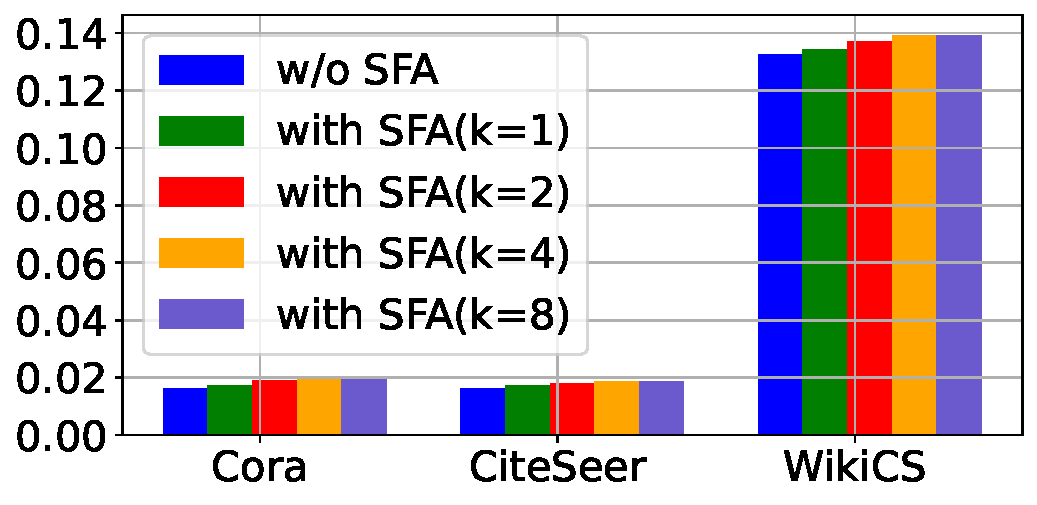
\includegraphics[width=1\textwidth]{picture/runningtime.pdf}
    \vspace{-0.7cm}
    \captionof{figure}{Running time per epoch in seconds. \label{fig:runningtime}}
	\end{minipage}
\begin{minipage}[c]{0.49\textwidth}
%\begin{figure}[t]
\vspace{0.05cm}
\centering
%\begin{minipage}[c]{0.21\textwidth}
\resizebox{\textwidth}{!}{
\begin{tabular}{l|c|c}
\toprule
\multirow{2}{*}{\textbf{Datasets}}  &    \multirow{2}{*}{{w/o SFA}}     & \multicolumn{1}{c}{{SFA}}  \\
& & $k= 1$  \\
\midrule
\textbf{Cora}       & $165$ &$172$  \\
\textbf{CiteSeer}   &$164$  &$173$  \\
\textbf{WikiCS}     &$1334$  &$1343$ \\
\bottomrule
\end{tabular}
}
\vspace{-0.12cm}
\captionof{table}{Running time per epoch in seconds.\label{tab:runningtime}}
\end{minipage}
		%
		%
%
\begin{minipage}[c]{\textwidth}
% \vspace{0.2cm}
 \resizebox{\textwidth}{!}{
    \begin{tabular}{cccc}
    \toprule
    Method &    SFA (ours)       &  SVD      & Random SVD \\
    \midrule
    Time   &    0.25 hour        &  12 hours & 1.2 hours  \\
    \bottomrule
    \end{tabular}
    }
    \captionof{table}{\label{tab:time_comp_svd}Running time on Ogb-arxiv.}
%\end{minipage}
%\end{figure}
%  
\end{minipage}
\end{minipage}
\begin{minipage}[c]{0.403\textwidth}
\resizebox{1\textwidth}{!}{
\begin{tabular}{l|cc}
\toprule
  \textbf{Ogb-arxiv}      & \textbf{Validation}     &\textbf{Test}\\
  \midrule
  MLP                                   & $57.6 \pm 0.2$     & $55.5 \pm 0.3$ \\
  Node2vec                              & $71.2 \pm 0.3$     & $70.0 \pm 0.3$ \\
  MVGLR                                 & $69.3 \pm 0.3$     & $68.2 \pm 0.2$ \\
  DGI                                   & $71.2 \pm 0.1$     & $70.3 \pm 0.1$ \\
  SUGRL                                 & $70.2 \pm 0.1$     & $69.3 \pm 0.2$ \\
  MERIT                                 & $67.2 \pm 0.1$     & $65.3 \pm 0.2$\\
  GRACE                                 & $71.4 \pm 0.5$     & $70.8 \pm 0.1$\\
  G-BT                                  & $71.1 \pm 0.3$     & $70.0 \pm 0.2$ \\
  COSTA                                  & $71.6 \pm 0.4$     & $71.0 \pm 0.4$ \\
 \rowcolor{LightCyan} SFA$_{\text{Info}}$           & \textcolor{blue}{$\bf 72.3 \pm 0.1$} & \textcolor{blue}{$\bf 71.6 \pm 0.4$} \\
  \bottomrule
    \end{tabular}
    }
\caption{Node classification.\label{tab:obgarxiv}}
\end{minipage}
\end{minipage}
%
%
%
%
%
\hspace{0.2cm}
\begin{minipage}[h]{0.33\textwidth}
\vspace{-0.5cm}
\centering
        \resizebox{0.95\textwidth}{!}{
             \setlength{\tabcolsep}{3pt}
    \begin{tabular}{lccc}
    \toprule
         \textbf{Method}        & \textbf{CIFAR10} & \textbf{CIFAR100} & \textbf{ImageNet-100}\\
         \hline
          SimCLR      &  $90.5$   &  $65.5$  & $76.8$ \\
         \rowcolor{LightCyan} SFA$_{\text{SimCLR}}$    &  \textcolor{blue}{$\mathbf{91.6}$}   &  \textcolor{blue}{$\mathbf{66.7}$} & $\textcolor{blue}{\mathbf{77.7}}$\\ 
         \midrule
         BalowTw      &  $92.0$   &  $69.7$ &  $80.0$  \\
         \rowcolor{LightCyan} SFA$_{\text{BT}}$   &  \textcolor{blue}{$\mathbf{92.5}$}   &  \textcolor{blue}{$\mathbf{70.4}$}   & \textcolor{blue}{$\mathbf{80.9}$} \\
         \midrule
 Siamese               &      $90.51$     &    $66.04$    &      $74.5$       \\
 \rowcolor{LightCyan}SFA$_{\text{Siamese}}$          &      \textcolor{blue}{$\mathbf{91.23}$}    &    \textcolor{blue}{\textbf{66.99}}    &     \textcolor{blue}{$\mathbf{75.6}$}     \\
 \midrule
 SwAV                  &      $89.17$     &    $64.88$    &     $74.0$       \\
 \rowcolor{LightCyan} SFA$_{\text{SwAV}}$            &      \textcolor{blue}{$\mathbf{90.12}$}     &    \textcolor{blue}{$\mathbf{65.82}$}    &      \textcolor{blue}{$\mathbf{74.8}$}       \\
    \bottomrule
    \end{tabular}
    }
    \vspace{-0.15cm}
    \caption{Image classification on CIFAR10, CIFAR100 and ImageNet-100.}
    \label{tab:image_result}

   \vspace{0.2cm}
    \resizebox{0.95\textwidth}{!}{
    \begin{tabular}{lccc}
\toprule
         \textbf{Method}        & \textbf{NCI1}   & \textbf{PROTEIN}  & \textbf{DD} \\
         \midrule
         GraphCL                   &$77.8 \pm 0.4$ &$74.3 \pm 0.4$ &${77.8 \pm 0.4}$ \\
         LP-Info                   &$75.8  \pm 1.2$   &$\textcolor{blue}{74.6 \pm 0.2}$ &$72.5 \pm 1.9$ \\
         JOAO                      &$\textcolor{blue}{78.0 \pm 0.4}$ &${74.5 \pm 0.4}$ &$\textcolor{blue}{77.5 \pm 0.5}$ \\
         SimGRACE                  &$77.4 \pm 1.0$   &$73.9 \pm 0.1$  &$77.3 \pm 1.1$ \\
         \rowcolor{LightCyan} SFA$_{\text{InfoNEC}} $     &$\textcolor{blue}{\mathbf{78.7 \pm 0.4}}$   &$\textcolor{blue}{\mathbf{75.4 \pm 0.4}}$  &$\textcolor{blue}{\mathbf{78.6 \pm 0.4}}$ \\
    \bottomrule%1.21 1.32
    \end{tabular}
    }
    \vspace{-0.15cm}
    \caption{Graph classification. \color{DarkBlue}{(SFA$_{\text{InfoNEC}}$ can be directly compared with  GraphCL.)} \label{tab:graphcls}}
% \vspace{-0.3cm}
 \vspace{0.2cm}
\resizebox{0.95\textwidth}{!}{
\begin{tabular}{cccccc}
\toprule
$\mathcal{A}_{G}$ & $\mathcal{A}_{F}$ & $\mathcal{A}_{F^*}$ & \textbf{Am-Comput.} & \textbf{Cora} & \textbf{CiteSeer} \\
\midrule 
$\times$     &$\times$ &$\times$         &$85.01$ &$80.04$   &$71.35$\\
$\checkmark$ &$\times$ &$\times$         &$87.25$ &$82.23$   &$74.56$\\
$\times$     &$\times$ &$\checkmark$     &$86.74$ &$84.19$   &$73.15$\\
\rowcolor{LightCyan}$\checkmark$ &$\times$ &$\checkmark$     &$\textcolor{blue}{\mathbf{88.74}}$ &$\textcolor{blue}{\mathbf{85.90}}$   &$\textcolor{blue}{\mathbf{75.05}}$\\
\midrule 
$\checkmark$     &$\checkmark$ &$\times$         &$87.55$& $83.35$&  $74.45$\\
\rowcolor{LightCyan} $\checkmark$     &$\checkmark$ &$\checkmark$    &$\textcolor{blue}{{88.69}}$ & $\textcolor{blue}{{84.50}}$&  $\textcolor{blue}{{74.70}}$\\
% $\times$     &$\times$ &$\checkmark$     &$86.74$ &$84.19$   &$73.15$\\
\bottomrule
\end{tabular}
}
\vspace{-0.15cm}
\caption{\label{tab:AblationStudy}Ablation study on different augmentation strategies: $\mathcal{A}_G$, $\mathcal{A}_F$ and $\mathcal{A}_{F^*}$.}
\end{minipage}
\vspace{-0.3cm}
\end{table*}



















% \begin{table*}[t]
% \begin{minipage}[c]{0.68\textwidth}
% \vspace{-0.5cm}
% \vskip 0.15in
% % \begin{center}
% % \begin{small}
% % \begin
% \centering
% \resizebox{\textwidth}{!}{
% \begin{tabular}{lcccccc}
% \toprule
% \textbf{Method}& \textbf{WikiCS} & \textbf{Am-Comput.} & \textbf{Am-Photo} & \textbf{Cora} & \textbf{CiteSeer} & \textbf{PubMed} \\
% \midrule 
% RAW fatures & $71.98 \pm 0.00$ & $73.81 \pm 0.00$ & $78.53 \pm 0.00$ & $64.61 \pm 0.22$ & $65.77 \pm 0.15$ & $82.02 \pm 0.26$\\
% DeepWalk & $74.35 \pm 0.06$ & $85.68 \pm 0.06$ & $89.44 \pm 0.11$ & $74.61 \pm 0.22$ & $50.77 \pm 0.15$ & $80.11 \pm 0.25$\\
% % DeepWalk + fts & $77.21 \pm 0.03$ & $86.28 \pm 0.07$ & $90.05 \pm 0.08$ & $87.70 \pm 0.04$ & $94.90 \pm 0.09$ \\
% \midrule
% DGI   & $75.35 \pm 0.14$ & $83.95 \pm 0.47$ & $91.61 \pm 0.22$  & $82.15 \pm 0.63$ & $69.51 \pm 0.52$  & $86.01 \pm 0.26$            \\
% MVGRL & $77.52 \pm 0.08$ & $87.52 \pm 0.11$ & $91.74 \pm 0.07$  & $83.11 \pm 0.12$ & $73.33 \pm 0.03$  & $84.27 \pm 0.04$            \\           
% GRACE & $78.19 \pm 0.48$ & $87.25 \pm 0.25$ & $92.15 \pm 0.25$  & $83.51 \pm 0.25$ & $73.63 \pm 0.20$ & $85.51 \pm 0.37$             \\
% GCA   & $78.35 \pm 0.05$ & $87.85 \pm 0.31$ & $92.49 \pm 0.16$  & $82.89 \pm 0.21$ & $72.89 \pm 0.13$ & $85.12 \pm 0.23$             \\
% SUGRL & $77.72 \pm 0.28$ & $88.83 \pm 0.23$  & $93.28 \pm 0.42$ & $83.47 \pm 0.55$ & $73.08 \pm 0.45$ & $84.91 \pm 0.31$\\
% MERIT & $77.92 \pm 0.43$ & $87.53 \pm 0.26$  & $93.12 \pm 0.42$ &$84.11  \pm 0.65$ &$74.34  \pm 0.43$ & $84.12 \pm 0.23$\\
% % \midrule 
% BGRL  & $79.11 \pm 0.62$ & $87.37 \pm 0.40$ & $91.57 \pm 0.44 $ & $83.77 \pm 0.57$ & $73.07 \pm 0.06$  \\
% G-BT  & $76.85 \pm 0.62$ & $86.86 \pm 0.33$ & $92.63 \pm 0.57$  & $83.63 \pm 0.44$ & $72.95 \pm 0.17$  \\
% % \midrule
% COSTA  &$79.12  \pm 0.02$ & $88.32 \pm 0.03$ & $92.56 \pm 0.45$  &$84.32  \pm 0.22$ & $72.92 \pm 0.31$ &$86.01\pm0.22$\\
% \midrule 
% \rowcolor{LightCyan} SFA$_{\text{BT}}$ & $\textcolor{blue}{\mathbf{80.22} \pm 0.05}$ & $\textcolor{blue}{88.14 \pm 0.15}$ & $\textcolor{blue}{92.83 \pm 0.14}$ & $\textcolor{blue}{84.10 \pm 0.01}$ & $\textcolor{blue}{73.73 \pm 0.03}$ \\
% \rowcolor{LightCyan} SFA$_{\text{InfoNCE}}$ & $\textcolor{blue}{79.98 \pm 0.05}$ & $\textcolor{blue}{\mathbf{89.24 \pm 0.27}}$ & $\textcolor{blue}{\mathbf{93.53 \pm 0.16}}$ & $\textcolor{blue}{\mathbf{86.43 \pm 0.01}}$ & $\textcolor{blue}{\mathbf{76.03 \pm 0.03}}$ & $\textcolor{blue}{\mathbf{86.29 \pm 0.13}}$\\
% % Supervised GCN & $77.19 \pm 0.12$ & $86.51 \pm 0.54$ & $92.42 \pm 0.22$ & $93.03 \pm 0.31$ & $95.65 \pm 0.16$ \\
% \bottomrule
% \end{tabular}
% }
% \caption{\label{tab:MainResultNodeClassifcation}Performance (accuracy (\%) and standard deviation) of node classification. Blue boldface indicates the best performance. \color{DarkBlue}{(Note that SFA$_{\text{InfoNEC}}$ and SFA$_{\text{BT}}$ can be directly compared to GRACE and G-BT.)}}
% % \end{sc}
% % \end{small}
% % \end{center}
% \vskip 0.2in

% \resizebox{0.3\textwidth}{!}{
% \begin{tabular}{l|cc}
% \toprule
%   \textbf{Ogb-arxiv}      & \textbf{Validation}     &\textbf{Test}\\
%   \midrule
%   MLP                                   & $57.6 \pm 0.2$     & $55.5 \pm 0.3$ \\
%   Node2vec                              & $71.2 \pm 0.3$     & $70.0 \pm 0.3$ \\
%   MVGLR                                 & $69.3 \pm 0.3$     & $68.2 \pm 0.2$ \\
%   DGI                                   & $71.2 \pm 0.1$     & $70.3 \pm 0.1$ \\
%   SUGRL                                 & $70.2 \pm 0.1$     & $69.3 \pm 0.2$ \\
%   MERIT                                 & $67.2 \pm 0.1$     & $65.3 \pm 0.2$\\
%   GRACE                                 & $71.4 \pm 0.5$     & $70.8 \pm 0.1$\\
%   G-BT                                  & $71.1 \pm 0.3$     & $70.0 \pm 0.2$ \\
%   COSTA                                  & $71.6 \pm 0.4$     & $71.0 \pm 0.4$ \\
%  \rowcolor{LightCyan} SFA$_{\text{InfoNCE}}$           & \textcolor{blue}{$\bf 72.3 \pm 0.1$} & \textcolor{blue}{$\bf 71.6 \pm 0.4$} \\
%   \bottomrule
%     \end{tabular}
%     }
% \caption{Node classification.}


% \end{minipage}





% \hspace{0.1cm}
% \begin{minipage}[c]{0.33\textwidth}

% \centering

%         \resizebox{\textwidth}{!}{
%              \setlength{\tabcolsep}{3pt}
%     \begin{tabular}{lccc}
%     \toprule
%          \textbf{Method}        & \textbf{CIFAR10} & \textbf{CIFAR100} & \textbf{ImageNet-100}\\
%          \hline
%           SimCLR      &  $90.5$   &  $65.5$  & $76.8$ \\
%          \rowcolor{LightCyan} SFA$_{\text{SimCLR}}$    &  \textcolor{blue}{$\mathbf{91.6}$}   &  \textcolor{blue}{$\mathbf{66.7}$} & $\textcolor{blue}{\mathbf{77.7}}$\\ 
%          \midrule
%          BalowTw      &  $92.0$   &  $69.7$ &  $80.0$  \\
%          \rowcolor{LightCyan} SFA$_{\text{BT}}$   &  \textcolor{blue}{$\mathbf{92.5}$}   &  \textcolor{blue}{$\mathbf{70.4}$}   & \textcolor{blue}{$\mathbf{80.9}$} \\
%          \midrule
%  Siamese               &      $90.51$     &    $66.04$    &      $74.5$       \\
%  \rowcolor{LightCyan}SFA$_{\text{Siamese}}$          &      \textcolor{blue}{$\mathbf{91.23}$}    &    \textcolor{blue}{\textbf{66.99}}    &     \textcolor{blue}{$\mathbf{75.6}$}     \\
%  \midrule
%  SwAV                  &      $89.17$     &    $64.88$    &     $74.0$       \\
%  \rowcolor{LightCyan} SFA$_{\text{SwAV}}$            &      \textcolor{blue}{$\mathbf{90.12}$}     &    \textcolor{blue}{$\mathbf{65.82}$}    &      \textcolor{blue}{$\mathbf{74.8}$}       \\
%     \bottomrule
%     \end{tabular}
%     }
%     \caption{Performance (accuracy (\%)) on image classification on three datasets (CIFAR10, CIFAR100 and ImageNet-100).}
%     \label{tab:image_result}

%     \centering
%     \resizebox{\textwidth}{!}{
%     \begin{tabular}{lccc}
% \toprule
%          \textbf{Method}        & \textbf{NCI1}   & \textbf{PROTEIN}  & \textbf{DD} \\
%          \midrule
%          GraphCL                   &$77.87 \pm 0.41$ &$74.39 \pm 0.45$ &${77.81 \pm 0.40}$ \\
%          LP-Info                   &$75.80  \pm 1.26$   &$\textcolor{blue}{74.64 \pm 0.22}$ &$72.55 \pm 1.98$ \\
%          JOAO                      &$\textcolor{blue}{78.07 \pm 0.47}$ &${74.55 \pm 0.41}$ &$\textcolor{blue}{77.58 \pm 0.54}$ \\
%          SimGRACE                  &$77.42 \pm 1.04$   &$73.97 \pm 0.09$  &$77.38 \pm 1.11$ \\
%          \rowcolor{LightCyan} SFA$_{\text{InfoNEC}} $     &$\textcolor{blue}{\mathbf{78.77 \pm 0.41}}$   &$\textcolor{blue}{\mathbf{75.49 \pm 0.45}}$  &$\textcolor{blue}{\mathbf{78.62 \pm 0.42}}$ \\
%     \bottomrule%1.21 1.32
%     \end{tabular}
%     }
%     \caption{Graph classification. \color{DarkBlue}{(SFA$_{\text{InfoNEC}}$ can be directly compared with  GraphCL.)} \label{tab:graphcls}}
% % \vspace{-0.3cm}
   

% \resizebox{\textwidth}{!}{
% \begin{tabular}{cccccc}
% \toprule
% $\mathcal{A}_{G}$ & $\mathcal{A}_{F}$ & $\mathcal{A}_{F^*}$ & \textbf{Am-Comput.} & \textbf{Cora} & \textbf{CiteSeer} \\
% \midrule 
% $\times$     &$\times$ &$\times$         &$85.01$ &$80.04$   &$71.35$\\
% $\checkmark$ &$\times$ &$\times$         &$87.25$ &$82.23$   &$74.56$\\
% $\times$     &$\times$ &$\checkmark$     &$86.74$ &$84.19$   &$73.15$\\
% \rowcolor{LightCyan}$\checkmark$ &$\times$ &$\checkmark$     &$\textcolor{blue}{\mathbf{88.74}}$ &$\textcolor{blue}{\mathbf{86.03}}$   &$\textcolor{blue}{\mathbf{76.05}}$\\
% \midrule 
% $\checkmark$     &$\checkmark$ &$\times$         &$87.55$& $83.35$&  $74.45$\\
% \rowcolor{LightCyan} $\checkmark$     &$\checkmark$ &$\checkmark$    &$\textcolor{blue}{{88.69}}$ & $\textcolor{blue}{{85.70}}$&  $\textcolor{blue}{{76.10}}$\\
% % $\times$     &$\times$ &$\checkmark$     &$86.74$ &$84.19$   &$73.15$\\
% \bottomrule
% \end{tabular}

% }
% \caption{\label{tab:AblationStudy}Ablation study on different augmentation strategies: $\mathcal{A}_G$, $\mathcal{A}_F$ and $\mathcal{A}_{F^*}$}
% \end{minipage}
% \end{table*}





% \begin{table}[t]
% \label{tab:obgResult}
% \centering
% \resizebox{0.3\textwidth}{!}{
% \begin{tabular}{l|cc}
%     \toprule
%   ogb-arxiv      & Validation     &Test\\
%   \midrule
%   MLP                                   & $57.6 \pm 0.12$     & $55.5 \pm 0.23$ \\
%   Node2vec                              & $71.2 \pm 0.13$     & $70.0 \pm 0.13$ \\
%   DGI                                   & $71.2 \pm 0.11$     & $70.3 \pm 0.16$ \\
%   GRACE                                 & $71.4 \pm 0.15$     & $70.8 \pm 0.11$\\
%   G-BT                                  & $71.1 \pm 0.13$     & $70.0 \pm 0.16$ \\
%   SFA$\_{\text{InfoNCE}}$           & $\bf 72.3 \pm 0.15$ & $\bf 71.6 \pm 0.11$ \\
%   \bottomrule
%     \end{tabular}
%     }
% \caption{Node classification on ogb-arxiv: Result of MLP,Node2Vec, and DGI is taken from official website.}

% \end{table}

Below we conduct  experiments on %several benchmark datasets to evaluate the effectiveness of the proposed method.
the node classification, node clustering, graph classification and image classification. 
For fair comparisons, we use the same experimental setup as the representative Graph SSL (GSSL) methods (\ie, GCA~\cite{zhu2020deep} and GRACE~\cite{zhu2021graph}). %, in order to perform a fair comparison with these methods.

\vspace{0.1cm}
\noindent\textbf{Datasets.}
We use five popular %benchmark 
datasets~\cite{zhu2020deep, zhu2021graph,velickovic2019deep}, including citation networks (Cora, CiteSeer) and social networks (Wiki-CS, Amazon-Computers, Amazon-Photo)~\cite{kipf2016semi,sinha2015overview,mcauley2015image, mernyei2020wiki}. 
For graph classification, we use NCI1, PROTEIN and DD \cite{dobson2003distinguishing,riesen2008iam}. For image classification we use CIFAR10/100~\cite{krizhevsky2009learning} and ImageNet-100~\cite{DBLP:conf/cvpr/DengDSLL009}.
See the \nameref{app:modelsetting}~section for details (supplementary material).

\vspace{0.1cm}
\noindent\textbf{Baselines.}
%To compare with previous  works, 
We  focus on three groups of SSL models. The first group includes traditional GSSL, \ie, Deepwalk~\cite{perozzi2014deepwalk}, node2vec~\cite{grover2016node2vec}, and  GAE~\cite{kipf2016variational}. The second group is contrastive-based GSSL, \ie,  %contrastive-based models including 
Deep Graph Infomax (DGI)~\cite{velickovic2019deep}, Multi-View Graph Representation Learning (MVGRL)~\cite{hassani2020contrastive}, GRACE~\cite{zhu2020deep}, GCA~\cite{zhu2021graph}, ~\cite{jin2021multi} SUGRL~\cite{mo2022simple}. The last group  %with objectives that %remove the need for
does not require explicit negative samples, \ie, Graph Barlow Twins(G-BT)~\cite{bielak2021graph} and BGRL~\cite{thakoor2021bootstrapped}. We also compare SFA with  COSTA~\cite{zhang2022costa} (GCL with feat. augmentation).

\vspace{0.1cm}
\noindent\textbf{Evaluation Protocol.} %For each experiment, 
We adopt the  %linear
evaluation from~\cite{velickovic2019deep, zhu2020deep, zhu2021graph}. Each model is trained in an unsupervised manner on the whole graph with node features. Then, we pass the raw features into the trained encoder to obtain   embeddings and train an $\ell_2$-regularized logistic regression classifier. Graph Datasets are randomly divided into 10\%, 10\%, 80\% for training, validation, and testing. We report the accuracy with mean/standard deviation over 20 random data splits.

\vspace{0.1cm}
\noindent \textbf{Implementation details} We use Xavier initialization for the GNN parameters and train the model with Adam optimizer. For node/graph classification, we use 2 GCN layers. The logistic regression classifier is trained with $5,000$ (guaranteed converge). We also use early stopping with a patience of 20 to avoid overfitting. We set the size of the hidden dimension of nodes to from ${128}$ to $512$. In clustering, we train a k-means clustering model. For the chosen hyper-parameters see Section~\ref{app:hyperparam}. We implement the major baselines using PyGCL~\cite{DBLP:journals/corr/pygcl}. The detailed settings of augmentation and contrastive objectives are in Table~\ref{tab:ModelAugSetting} of Section~\ref{app:modelsetting}. 

%Move to appendix%

% \subsection{Implementation Details}
% We implement our approach based on PyTorch~\cite{DBLP:journals/corr/pytorch}. We initialize the parameters using Xavier initialization and train the model using Adam optimizer. For node classification, we follow our major baseline GRACE and set the number of GCN layers to 2. The logistic regression classifier is trained with $5000$ epochs to guarantee a converge. We also use early stopping with a patience of 20 to avoid overfitting. Finally, we set the size of the hidden dimension of nodes to from ${128}$ to $512$. For the chosen hyper-parameters see Appendix~\ref{app:hyperparam}. We implement the major baselines using PyGCL~\cite{DBLP:journals/corr/pygcl}, an open-source graph contrastive learning framework, and use the hyper-parameters described in their original paper. The detailed settings of augmentation and contrastive objectives are in Table~\ref{tab:ModelAugSetting} of Appendix~\ref{app:modelsetting}. Apart from Wiki-CS adopting the public split, other datasets are randomly divided into 10\%, 10\%, 80\% for training, validation, and testing.
 

\subsection{Main Results}
\noindent\textbf{Node Classification\footnote{Implementation and evaluation are based on  PyGCL \cite{DBLP:journals/corr/pygcl}: \url{https://github.com/PyGCL/PyGCL}.}.}
We employ  node classification as a downstream task to showcase  SFA. The default contrastive objective is InfoNCE or the BT loss. Table~\ref{tab:MainResultNodeClassifcation} shows that SFA consistently achieves the best results on all datasets. Notice that the graph-augmented  GSSL methods, including GSSL with SFA, significantly outperform the traditional methods, illustrating the importance of data augmentation in GSSL. Moreover, we find that the performance of GCL methods (\ie, GRACE, GCA, DGI, MVGRL) improves by a large margin when integrating with SFA (\eg, major baseline, GRACE, yields 3\% and 4\% gain on  Cora and Citeseer), which shows that SFA  is complementary to graph augmentations. SFA  
 also works with the BT loss and  improves its performance.




% \begin{table}[t]
% \caption{Classification accuracies for different power iteration.}

% \vskip 0.15in
% \begin{center}
% \begin{small}
% \begin{sc}
% \begin{tabular}{c|ccc}
% \toprule
% \toprule
% \textbf{Power Iter}. & \textbf{Am-Computer} & \textbf{Cora} & \textbf{CiteSeer} \\
% \midrule 
% k = 0 &$86.63$  &$83.04$   &$71.35$\\
% k = 1 &$\mathbf{88.83}$    &$\mathbf{86.34}$   &$73.56$\\
% k = 2 &$88.64$  &$85.29$   &$\mathbf{76.15}$\\
% k = 4 &$88.72$  &$85.53$   &$75.85$\\
% k = 8 &$88.67$  &$86.23$   &$76.35$\\
% \bottomrule
% \bottomrule
% \end{tabular}
% \end{sc}
% \end{small}
% \end{center}
% \end{table}
% \begin{table}[t]
% % \caption{Ablation study on graph augmentation $\mathcal{A}_G$ and feature augmentation $\mathcal{A}_F$.}
% \vskip 0.15in
% \begin{center}
% \begin{small}
% \begin{sc}
% \begin{minipage}[t]{0.47\textwidth}
% \caption{Ablation study on different augmentation strategies, \ie, $\mathcal{A}_G$, $\mathcal{A}_F$ and $\mathcal{A}_{F^*}$}
% \resizebox{\textwidth}{!}{
% \begin{tabular}{cccccc}
% \toprule
% $\mathcal{A}_{G}$ & $\mathcal{A}_{F}$ & $\mathcal{A}_{F^*}$ & \textbf{Am-Computer} & \textbf{Cora} & \textbf{CiteSeer} \\
% \midrule 
% $\times$     &$\times$ &$\times$         &$85.01$ &$80.04$   &$71.35$\\
% $\checkmark$ &$\times$ &$\times$         &$87.25$ &$82.23$   &$74.56$\\
% $\times$     &$\times$ &$\checkmark$     &$86.74$ &$84.19$   &$73.15$\\
% \rowcolor{LightCyan}$\checkmark$ &$\times$ &$\checkmark$     &$\textcolor{blue}{\mathbf{88.74}}$ &$\textcolor{blue}{\mathbf{86.03}}$   &$\textcolor{blue}{\mathbf{76.05}}$\\
% \midrule 
% $\checkmark$     &$\checkmark$ &$\times$         &$87.55$& $83.35$&  $74.45$\\
% \rowcolor{LightCyan} $\checkmark$     &$\checkmark$ &$\checkmark$    &$\textcolor{blue}{{88.69}}$ & $\textcolor{blue}{{85.70}}$&  $\textcolor{blue}{{76.10}}$\\
% % $\times$     &$\times$ &$\checkmark$     &$86.74$ &$84.19$   &$73.15$\\
% \bottomrule
% \end{tabular}
% \label{tab:AblationStudy}
% }
% \end{minipage}
% \hspace{0.2cm}
% \begin{minipage}[t]{0.47\textwidth}
% \caption{Classification accuracy \wrt different $k$ of the incomplete power iteration.}
% \label{tab:EffectofK}
% \resizebox{\textwidth}{!}{
% \begin{tabular}{cccc}
% \toprule
% \textbf{Power Iter}. & \textbf{Am-Computer} & \textbf{Cora} & \textbf{CiteSeer} \\
% \midrule 
% $k=0$ &$87.25$  &$83.04$   &$71.35$\\
% $k=1$ &$\mathbf{\textcolor{blue}{ 88.83}}$    &$\textcolor{blue}{\mathbf{86.34}}$   &$73.56$\\
% $k=2$ &$\textcolor{blue}{88.72}$  &$\textcolor{blue}{85.59}$   &$\textcolor{blue}{\mathbf{76.35}}$\\
% $k=4$ &$88.64$  &$85.29$   &${75.15}$\\
% $k=8$ &$88.27$  &$85.23$   &$\textcolor{blue}{75.40}$\\
% \bottomrule
% \end{tabular}
% }
% \end{minipage}

% \end{sc}
% \end{small}
% \end{center}
% \vskip -0.35in
% \end{table}

% \begin{figure*}[h]
% \vspace{-0.3cm}
% %\vskip 0.2in
% % \centering
% \begin{minipage}[c]{0.68\textwidth}
% \begin{minipage}[c]{0.32\textwidth}
% 
\includegraphics[width=\columnwidth]{picture/fig1.pdf}
% % \vspace{-0.7cm}
% \caption{Spectrum of $\tilde{\mathbf{H}}$ when training on Cora dataset with SFA.}
% \label{fig:Eigen1}
% \end{minipage}
% \hspace{1px}
% \begin{minipage}[c]{0.32\textwidth}
% 
\includegraphics[width=\columnwidth]{picture/fig2.pdf}
% % \vspace{-0.7cm}
% \caption{Spectrum of $\mathbf{H}$ when training in Cora dataset without SFA.}
% \label{fig:Eigen2}
% \end{minipage}
% \hspace{1px}
% \begin{minipage}[c]{0.32\textwidth}
%     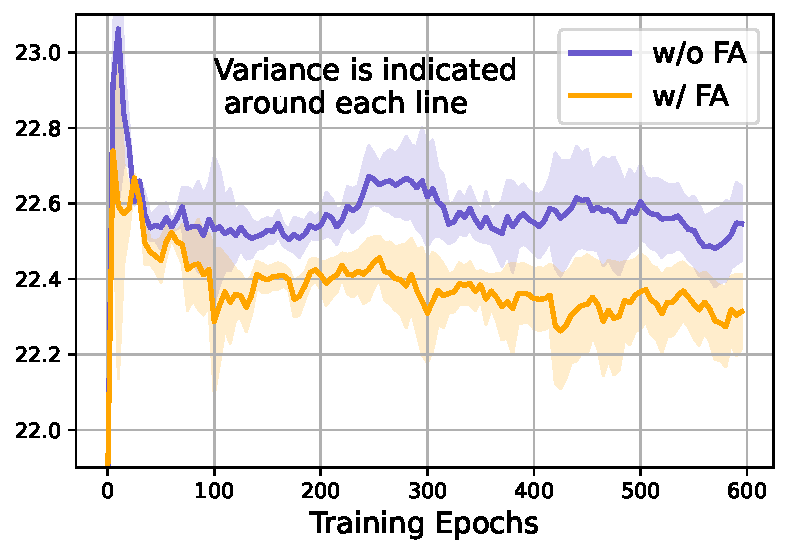
\includegraphics[width=\columnwidth]{picture/alignment.pdf}
%     % \vspace{-0.7cm}
%     \caption{Alignment of  feature maps of two views (the lower, the better).}
%     \label{fig:EigenAlign}
% \end{minipage}
% \begin{minipage}[c]{\textwidth}
% \vspace{2px}
%     \begin{subfigure}[b]{0.32\textwidth}
%     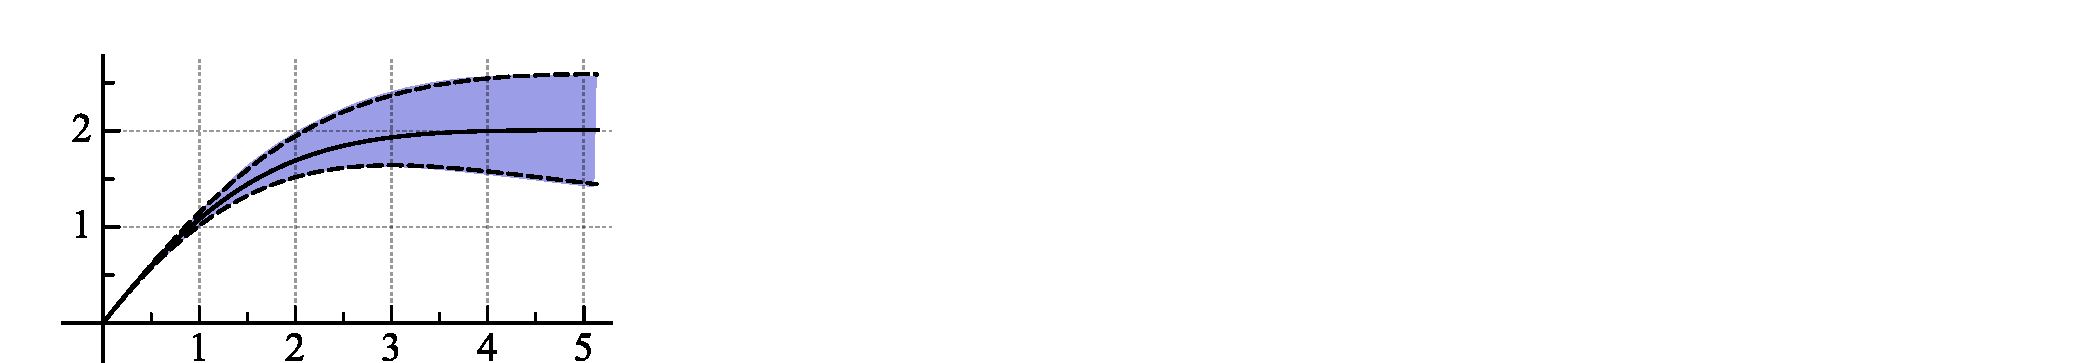
\includegraphics[width=\textwidth]{picture/v1.pdf}
%     \caption{\label{fig:v1}  SFA}
%     \end{subfigure}
%     \hspace{1px}
%     \begin{subfigure}[b]{0.32\textwidth}
%     
\includegraphics[width=\textwidth]{picture/v2.pdf}
%     \caption{\label{fig:v2} MaxExp(F)}
%     \end{subfigure}
%     \hspace{1px}
%     \begin{subfigure}[b]{0.32\textwidth}
%     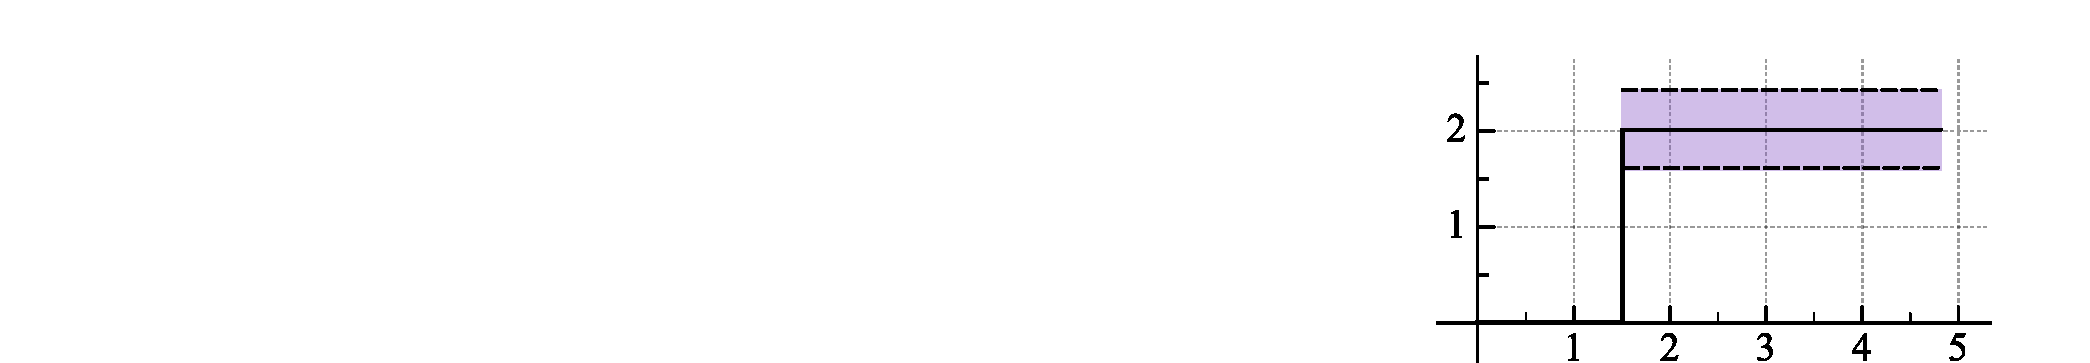
\includegraphics[width=\textwidth]{picture/v3.pdf}
%     \caption{\label{fig:v3} Grassman}
% \end{subfigure}
% \vspace{-9px}
% \caption{Spectrum augmentation variants (dashed lines: variance of injected noise).}\label{fig:new_var}
% \end{minipage}
% \end{minipage}
% \hspace{15px}

% % \vskip -0.10in
% \vspace{-0.5cm}
% \end{figure*}

%\begin{figure}[t]
%\centering
%\begin{minipage}[c]{0.21\textwidth}
%\resizebox{\textwidth}{!}{
%\begin{tabular}{l|c|c}
%\toprule
%\multirow{2}{*}{\textbf{Datasets}}  &    \multirow{2}{*}{{w/o SFA}}     & \multicolumn{1}{c}{{SFA}}  \\
%& & $k= 1$  \\
%\midrule
%\textbf{Cora}       & $0.0165$ &$0.0172$  \\
%\textbf{CiteSeer}   &$0.0164$  &$0.0173$  \\
%\textbf{WikiCS}     &$0.1334$  &$0.1343$ \\
%\bottomrule
%\end{tabular}
%}

%\captionof{table}{Running time per epoch in seconds.\label{tab:runningtime}}
%    \end{minipage}
%\begin{minipage}[c]{0.25\textwidth}
%    \centering
%    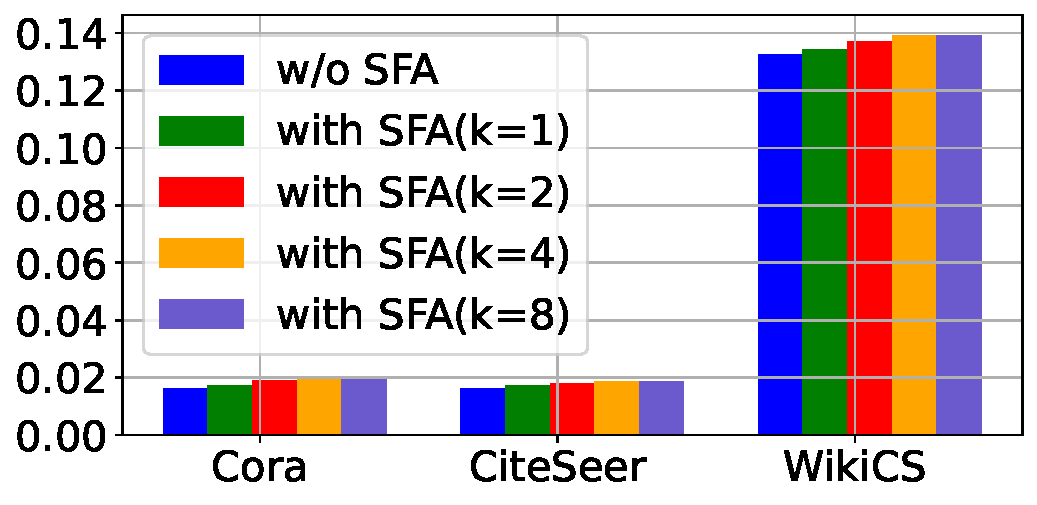
\includegraphics[width=\textwidth]{picture/runningtime.pdf}
%    %\vspace{-0.3cm}
%    \caption{Running time per epoch in seconds. \label{fig:runningtime}}
%   
%\end{minipage}%
%
%\begin{minipage}[c]{0.4\textwidth}
% \resizebox{\textwidth}{!}{
%    \begin{tabular}{cccc}
%    \toprule
%    Method &    SFA (ours)       &  SVD      & Random SVD \\
%    \midrule
%    Time   &    0.25 hour        &  12 hours & 1.2 hours  \\
%    \bottomrule
%    \end{tabular}
%    }
%    \captionof{table}{\label{tab:time_comp_svd}Running time in ogb-arxiv}
%\end{minipage}
%\end{figure}

\vspace{0.1cm}
\noindent\textbf{Graph Classification.}
By adopting the graph-level GNN encoder, SFA can be used for the graph-level pre-taining. %We present the graph classification result on three datasets. 
Thus, we compare SFA with graph augmentation-based models (\ie, GarphCL \citep{DBLP:conf/nips/YouCSCWS20}, JOAO~\citep{DBLP:conf/icml/YouCSW21}) and augmentation-free models (\ie, SimGrace~\cite{DBLP:conf/www/XiaWCHL22}, LP-Info~\cite{DBLP:conf/wsdm/YouCWS22}). Table~\ref{tab:graphcls} shows that SFA outperforms all baselines on the three datasets.

\vspace{0.1cm}
\noindent\textbf{Image Classification\footnote{Implementation/evaluation are based on Solo-learn~\cite{JMLR:v23:21-1155}: \url{https://github.com/vturrisi/solo-learn}.$\!\!\!\!$}.}
As SFA perturbs the spectrum of feature maps, it is also applicable to %a variety of CL domains, % in non-graph domains 
%\eg, 
the image domain. Table~\ref{tab:image_result}  presents the top-1 accuracy on CIFAR10/100 and ImageNet-100. See also the \nameref{sec:impl} (supp. material). 


%\subsection{Timing}
%\label{sec:timing}
\vspace{0.1cm}
\noindent\textbf{Runtimes.}  
Table~\ref{tab:runningtime} and Fig.~\ref{fig:runningtime} show SFA incurs a negligible runtime overhead  (few matrix-matrix(vector) multiplications). % while improving results. %SVD-based rebalancing is  slow. %Below, we present the running times per epoch in seconds.
The cost of SFA for $k\!<\!8$ iterations %(Fig. \ref{fig:runningtime}) 
is negligible.

% \begin{table}[H]
% \caption{Running time per epoch in seconds.}
% \label{tab:runingtime}
% \centering
% % \begin{minipage}[c]{0.45\textwidth}

% \resizebox{0.4\textwidth}{!}{
% \begin{tabular}{l|c|cccc}
% \toprule
% \multirow{2}{*}{\textbf{Datasets}}  &    \multirow{2}{*}{{w/o SFA}}     & \multicolumn{4}{c}{{with SFA}}  \\
% & & $k= 1$ & $k=2$   & $k=4$   & $k=8$ \\
% \midrule
% \textbf{Cora}       & $0.0165$ &$0.0172$ &$0.0189$ & $0.0194$ & $0.0229$  \\
% \textbf{CiteSeer}   &$0.0164$  &$0.0173$ & $0.0179$ &$0.0188$ & $0.0232$ \\\textbf{WikiCS}     &$0.1334$  &$0.1343$ & $0.1370$ &$0.1393$ &$0.1416$ \\
% \bottomrule
% \end{tabular}
% }
% % \end{minipage}
% \end{table}


% \begin{table}[t]
%     \centering
%     \resizebox{0.4\textwidth}{!}{
%     \begin{tabular}{cccc}
%     \toprule
%     Method &    SFA (ours)       &  SVD      & Random SVD \\
%     \midrule
%     Time   &    0.25 hour        &  12 hours & 1.2 hours  \\
%     \bottomrule
%     \end{tabular}
%     }
%     \caption{\label{tab:time_comp_svd}Running time in ogb-arxiv}
% \end{table}

%\vspace{-0.5cm}
%\vspace{0.1cm}
%\noindent\textbf{Fast Spectrum Balancing.} 
To rebalance the spectrum, choices for a push-forward function whose curve gets  flatter as singular values get larger  are many but they require SVD to rebalance singular values directly. %, and reassemble the feature matrix from rebalanced singular values and singular vectors. 
The complexity of SVD is $\mathcal{O}(nd_h^2)$ for $n\!\gg\!d_h$, which is costly in GCL as  SVD has to be computed per mini-batch (and SVD is unstable in back-prop. due to non-simple singular values ).  Table~\ref{tab:time_comp_svd} shows the runntime on  Ogb-arixv. 

\subsection{Analysis on Spectral Feature Augmentation}
\label{sec:spectrum}
%\vspace{0.1cm}
\noindent\textbf{Improved Alignment.}
We show that SFA improves the alignment of two views during training. Let $\mathbf{H}^\alpha$ and $\mathbf{H}^\beta$ ($\widetilde{\mathbf{H}}^\alpha$ and $\widetilde{\mathbf{H}}^\beta$) denote the feature maps of two views without (with) applying SFA. The alignment is computed by $\|\mathbf{H}^\alpha -\mathbf{H}^\beta\|^2_F$ (or $\|\tilde{\mathbf{H}}^\alpha -\tilde{\mathbf{H}}^\beta\|^2_F$). Fig.~\ref{fig:EigenAlign}  shows that SFA achieves better alignment. See also the \nameref{sec:moreresult}.

\vspace{0.1cm}
\noindent\textbf{Empirical Evolution of Spectrum.}
Fig.~\ref{fig:Eigen1} (Cora) shows how the singular values of  features maps ${\mathbf{H}}$ (without SFA) and $\tilde{\mathbf{H}}$ (with SFA) evolve. As training progresses, the gap between consecutive singular values gradually decreases due to SFA. The leading components of spectrum (where the signal is) become more balanced: empirical results match Prop.~\ref{prop:FeatureAug} \&  \ref{prop:PowerIter1}.

\vspace{0.1cm}
\noindent\textbf{Ablations on Augmentations.}
Below, %we conduct an ablation study on Cora, Citeseer and Am-Computer. 
we compare graph augmentation $\mathcal{A}_G$, channel feature augmentation $\mathcal{A}_F$ (random noise  added to embeddings directly) and the spectral feature augmentation $\mathcal{A}_{F^*}$.  Table~\ref{tab:AblationStudy} shows that using $\mathcal{A}_G$ or $\mathcal{A}_{F^*}$ alone  improves performance. For example, $\mathcal{A}_G$ yields 2.2\%, 2.2\% and 3.2\% gain on Am-Computer, Cora, and CiteSeer. $\mathcal{A}_{F^*}$ yields 1.7\%, 4.1\% and 1.8\% gain on  Am-Computer, Cora, and CiteSeer. Importantly, when both $\mathcal{A}_G$ and $\mathcal{A}_{F^*}$ are applied, the gain is \textbf{3.7}\%, \textbf{6.0}\% and \textbf{4.8}\% on Am-Computer, Cora, and CiteSeer over ``no augmentations''. Thus, SFA is complementary to existing graph augmentations. We also notice that $\mathcal{A}_{F^*}$ with $\mathcal{A}_G$ outperforms $\mathcal{A}_{F}$ with $\mathcal{A}_G$ by 1.1\%, 2.4\% and 1.7\%, which highlights the benefit of SFA.



\vspace{0.1cm}
\noindent\textbf{Effect of Number of Iterations ($k$).}
Below, we analyze how $k$ in Eq.~\eqref{equ:FeatureAug} influences the performance. We set $k \in \{0, 1, 2, 4, 8\}$ in our model with the InfoNCE loss on Cora, Citeseer and Am-Computer. The case of $k=0$ means that no power iteration is used, \ie, the solution simplifies to the feature augmentation by subtracting from $\mathbf{H}$ perturbation  $\mathbf{H}\mathbf{r}^{(0)}{\mathbf{r}^{(0)}}^\top\!\!/\|\mathbf{r}^{(0)}\|_2^2$ with random $\mathbf{r}^{(0)}$. 
Table~\ref{tab:EffectofK} shows that without power iteration, the performance of the model drops , \ie, 1.5\%, 3.3\% and 2.2\% on  Am-Comp., Cora and Citeseer. 
%

\vspace{-0.1cm}
\begin{tcolorbox}[width=1.0\linewidth, colframe=blackish, colback=beaublue, boxsep=0mm, arc=2mm, left=2mm, right=2mm, top=2mm, bottom=2mm]
The best gain in Table ~\ref{tab:EffectofK} is achieved for $1\leq k\leq 2$. This is consistent with Prop. \ref{prop:PowerIter1}, Fig. \ref{fig:sim2} and \ref{fig:sim3}, which show that the spectrum balancing effect (approximately flat region of $\phi$) and significant spectrum  augmentation (indicated by the large deviation in Fig. \ref{fig:sim2}) are achieved only when the power iteration is incomplete (low $k$, \ie, $1\leq k\leq 2$).
\end{tcolorbox}
\vspace{-0.1cm}
%\vspace{-0.5cm}

\begin{figure}
\begin{minipage}[c]{0.5\textwidth}
\begin{minipage}[b]{0.47\textwidth}

\includegraphics[width=\columnwidth]{picture/fig1.pdf}
\vspace{-0.7cm}
\caption{Spectrum of $\tilde{\mathbf{H}}$ when training on Cora with SFA.}
\vspace{0.2cm}
\label{fig:Eigen1}
\end{minipage}
\hspace{2px}
% \begin{minipage}[c]{0.32\textwidth}
% 
\includegraphics[width=\columnwidth]{picture/fig2.pdf}
% % \vspace{-0.7cm}
% \caption{Spectrum of $\mathbf{H}$ when training in Cora dataset without SFA.}
% \label{fig:Eigen2}
% \end{minipage}
% \hspace{1px}
\begin{minipage}[b]{0.48\textwidth}
    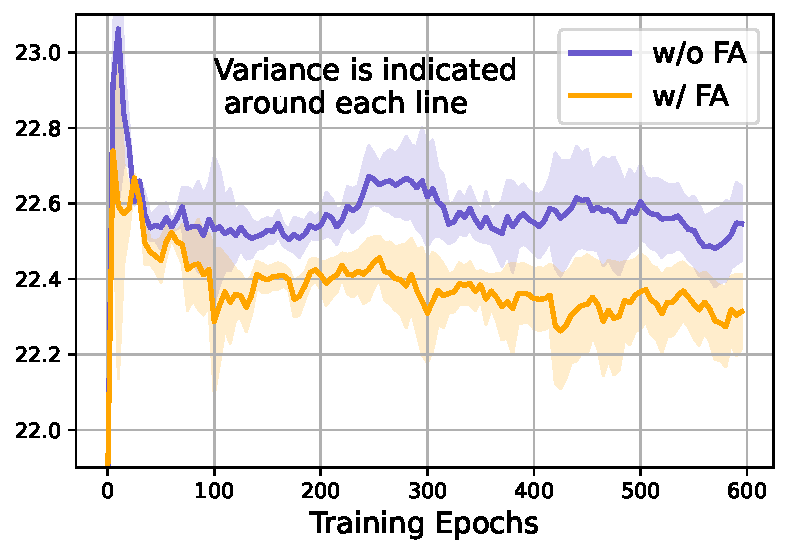
\includegraphics[width=\columnwidth]{picture/alignment.pdf}
    \vspace{-0.7cm}
    \caption{Alignment of  f. maps of two views (lower is better).}
    \label{fig:EigenAlign}
    \vspace{0.2cm}
\end{minipage}
\end{minipage}
\begin{minipage}[c]{0.5\textwidth}
\vspace{2px}
    \begin{subfigure}[b]{0.32\textwidth}
     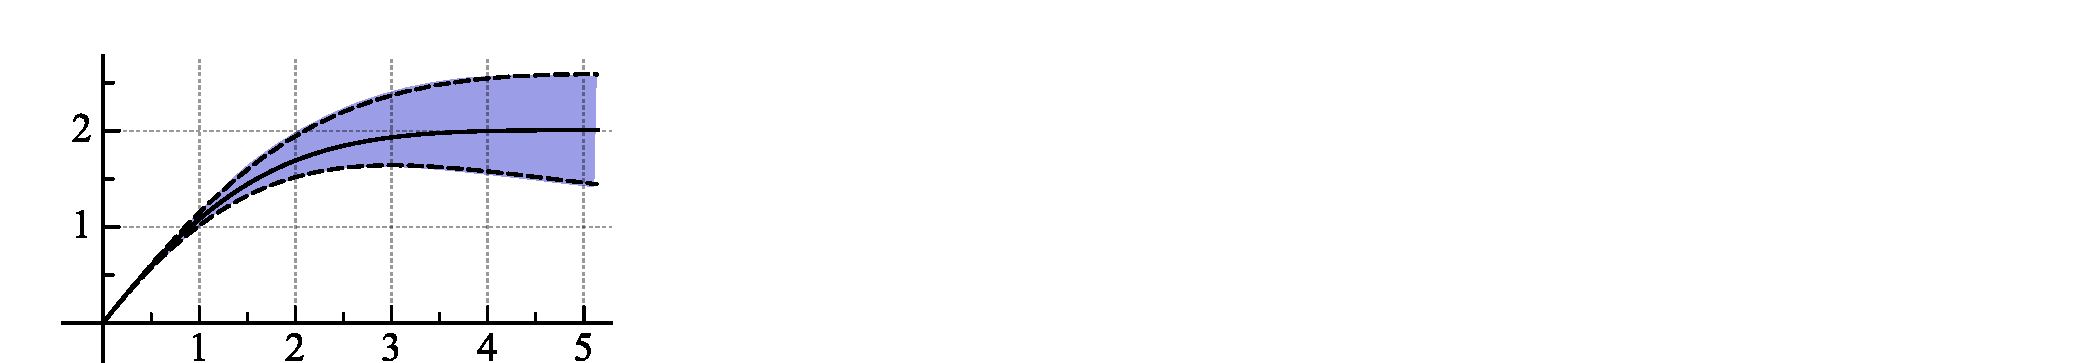
\includegraphics[width=\textwidth]{picture/v1.pdf}
    \caption{\label{fig:v1}  SFA}
    \end{subfigure}
    \hspace{1px}
    \begin{subfigure}[b]{0.32\textwidth}
    
\includegraphics[width=\textwidth]{picture/v2.pdf}
    \caption{\label{fig:v2} MaxExp(F)}
    \end{subfigure}
    \hspace{1px}
    \begin{subfigure}[b]{0.32\textwidth}
    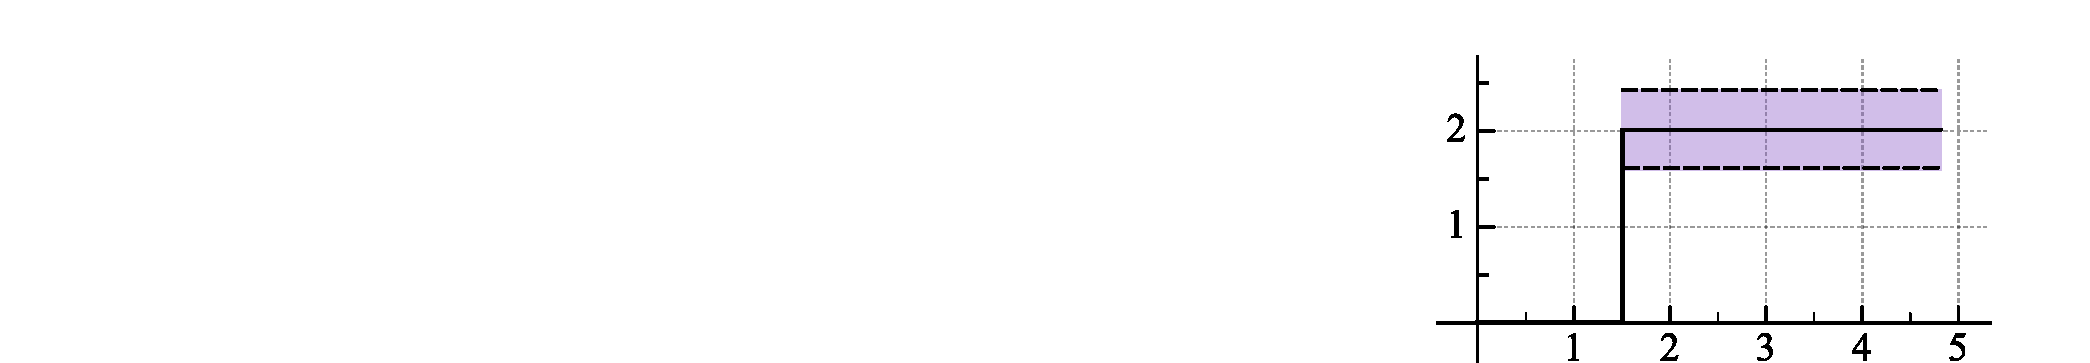
\includegraphics[width=\textwidth]{picture/v3.pdf}
    \caption{\label{fig:v3} Grassman}
\end{subfigure}
\vspace{-9px}
\vspace{-0.2cm}
\caption{Spectrum augmentation variants (dashed lines: injected noise var.) Power  Norm. \& Power Norm.$^*$ resemble (b) and (a).}\label{fig:new_var}
\end{minipage}
\vspace{-0.3cm}
\end{figure}


%\vspace{0.1cm}
\noindent\textbf{Robustness to Noisy Features.}
Below we check on Cora and CiteSeer if GCL with SFA is robust to noisy node features in node classification setting. 
%To empirically verify SFA is robustness to the noise feature
We draw noise $\Delta\mathbf{x} \sim \mathcal{N}(0,\mathbf{I})$ and inject it into the original node features as   $\mathbf{x}+\epsilon\Delta\mathbf{x}$, where $\epsilon\!\geq\!0$ controls the noise intensity.  Table~\ref{tab:nosiy_feature} shows that  SFA is robust to the noisy features. SFA partially balances the spectrum (Fig~\ref{fig:sim2} and~\ref{fig:simulation} ) of leading singular components where the signal lies, while non-leading components where the noise resides are left mostly unchanged by SFA.  %Non-leading components are left untouched as they may still carry some signal.

\vspace{0.1cm}
\noindent\textbf{Other Variants of Spectral Augmentation.} Below, we experiment with other ways of performing spectral augmentation. Figure \ref{fig:new_var} shows three different push-forward functions: our SFA, MaxExp(F) \cite{maxexp} and Grassman feature maps   \cite{mehrtash_dict_manifold}. As MaxExp(F) and Grassman do not inject any spectral noise, we equip them with explicit noise injectors. To determine what is the best form of such an operator, we vary (i) where the noise is injected, (ii) profile of balancing curve. As  the push-forward profiles of SFA and MaxExp(F) are similar (Figure \ref{fig:new_var}), we implicitly inject the noise into MaxExp(F) along the non-leading singular values (\cf leading singular values of SFA).

\vspace{0.1cm}
\noindent{\em MaxExp(F)} is only defined for symmetric-positive definite matrices. We extend it to feature maps by:

\vspace{-0.3cm}
\begin{equation}
\begin{aligned}
         \widetilde{\mathbf{H}} \!=\! \mathbf{H}\mathbf{B}\big(\mathbf{I}-(\mathbf{I}-\mathbf{A}/\text{Tr}(\mathbf{A}))^{\eta+\Delta\eta}\big),
    \end{aligned}
    \label{eq:maxexp}
    %\vspace{-0.1cm}
\end{equation}
%
where $\mathbf{A}=(\mathbf{H}^\top\mathbf{H})^{0.5}$ and $\mathbf{B}=(\mathbf{H}^\top\mathbf{H})^{-0.5}$ are obtained via highly-efficient Newton-Schulz iteration. We draw the random noise  $\Delta\eta\!\sim\!\alpha\mathcal{N}(0,1)$ for each $\mathbf{H}$ and control the variance by $\alpha\!>\!0$. We round $\eta+\Delta\eta$ to the nearest integer (MaxExp(F) requires an integer for fast matrix exponentiation) and ensure the integer is greater than zero. See  the \nameref{sec:maxexp}~section for details.



\vspace{0.1cm}
\noindent
{\em{Matrix Square Root}} is similar to MaxExp(F)  but the soft function flattening the spectrum is replaced with a matrix square root push-forward function. {\em Power Norm.} yields:
%\begin{equation}
%  \!\!\!\!\text{PowerNorm}(\sigma_i; \beta, \Delta\boldsymbol{\beta})=(1-\beta-\Delta{\beta})\sigma_i^{0.5}+(\beta+\Delta{\beta})\sigma_i^{0.75},
%\end{equation}
%
%

\vspace{-0.3cm}
\begin{equation}
\begin{aligned}
\widetilde{\mathbf{H}}&=\mathbf{H}\mathbf{B}\,\text{PowerNorm}(\mathbf{A}; \beta\!+\!\Delta{\beta}),
\end{aligned}
\end{equation}
%
%
where $0\leq\beta\!+\Delta{\beta}\!\leq 1$ controls the steepness of the balancing push-forward curve. $\Delta{\beta}$ is %a random vector 
drawn from the Normal distribution (we choose the best aug. variance). {\em Power Norm.$^*$} is:
%\begin{equation}
%  \!\!\!\!\text{PowerNorm}(\sigma_i; \beta, \Delta\boldsymbol{\beta})=(1-\beta-\Delta{\beta})\sigma_i^{0.5}+(\beta+\Delta{\beta})\sigma_i^{0.75},
%\end{equation}
%
%
\vspace{-0.3cm}
\begin{align}
\!\!\!\!\widetilde{\mathbf{H}}&=\mathbf{H}\mathbf{B}\big( (1-\beta\!-\!\Delta{\beta})\mathbf{A}^{0.5} +(\beta\!+\!\Delta{\beta})\mathbf{A}^{0.5}\mathbf{A}^{0.25}\big)\nonumber\\
&=\mathbf{H}\mathbf{B}\,\text{PowerNorm}(\mathbf{A}; \beta\!+\!\Delta{\beta}),
\end{align}
\vspace{-0.3cm}
%
%

\noindent
where $0\!\leq\!1\!+\Delta{\beta}^*\!\leq\!2$,  $\Delta{\beta}^*$ is drawn  from the Normal dist. 
%
%
% per sample. 
%We ensure that $0\leq\beta+\Delta{\beta}\leq 1$ and $0\leq 1-\beta-\Delta{\beta}\leq 1$. In practice, we achieve the above function by Newton-Schulz iterations. Specifically, we have:
%
%\begin{equation}
%\begin{aligned}
%\widetilde{\mathbf{H}}&=\mathbf{H}\mathbf{B}\big( (1-\beta\!-\!\Delta{\beta})\mathbf{A}^{0.5} +(\beta\!+\!\Delta{\beta})\mathbf{A}^{0.5}\mathbf{A}^{0.25}\big)\\
%&=\mathbf{H}\mathbf{B}\,\text{PowerNorm}(\mathbf{A}; \beta\!+\!\Delta{\beta}),
%\end{aligned}
%\end{equation}
%
 $\mathbf{A}^{0.5}$ and $\mathbf{A}^{0.25}\!=\!\left(\mathbf{A}^{0.5}\right)^{0.5}\!$ are obtained by Newton-Schulz iterations. See  \nameref{sec:pnnoise} for details.



\vspace{0.1cm}
\noindent{\em Grassman feature maps } can be obtained as:

\vspace{-0.3cm}
\begin{equation}
\begin{aligned}
         \widetilde{\mathbf{H}} \!=\! \mathbf{H}\mathbf{B}\big(\mathbf{V}\text{Flat}(\mathbf{\Lambda}; \kappa)\mathbf{V}^\top\big),
    \end{aligned}
    \label{eq:grass}
    %\vspace{-0.1cm}
\end{equation}
%
where $\text{Flat}(\cdot; \kappa)$ sets $\kappa\!>\!0$ leading singular values to $1+\Delta\boldsymbol{\kappa}$ (the rest is 0), and $\Delta\boldsymbol{\kappa}\!\sim\!\alpha\mathcal{N}(0,\mathbf{I})$. In experiments we use SVD and random SVD (injects itself some noise) to produce $\mathbf{V}$ and $\mathbf{\Lambda}$ from $\mathbf{A}$. See  \nameref{sec:grass} for details.

Table \ref{tab:spec_aug} shows that SFA outperforms MaxExp(F), Power Norm., Power Norm.$^*$ and Grassman. As SFA  augments parts of spectrum where signal resides (leading singular values) which is better than  augmenting non-leading singular values  (some noise may reside there) as in MaxExp(F). As Grassman  binarizes spectrum, it may reject some useful signal at the boundary between leading and non-leading singular values. Finally,  \nameref{sec:mp} model reduces the spectral gap, thus rebalances the spectrum (also non-leading part).




% \begin{table}[t]
%     \centering
%     \begin{tabular}{c|ccc}
% \toprule
% \toprule
% $k$ & \textbf{Am-Computer} & \textbf{Cora} & \textbf{CiteSeer} \\
% \midrule 
% k = 0 &  &$83.04$   &$71.35$\\
% k = 1 &  &$86.34$   &$72.56$\\
% k = 2 &  &$85.29$   &$76.15$\\
% k = 4 &  &$85.53$   &$76.25$\\
% k = 8 &  &$86.23$   &$76.05$\\
% \bottomrule
% \bottomrule
% \end{tabular}
%     \caption{Caption}
%      
% \end{table}


% \subsection{Effect of $\eta$}

\begin{table}[t]
\centering
\begin{minipage}[c]{0.42\textwidth}
\centering
    \resizebox{1\textwidth}{!}{
    \hspace{0.05cm}
    \begin{tabular}{cccc}
    \toprule
    \textbf{Power Iteration} & \textbf{Am-Computer} & \textbf{Cora} & \textbf{CiteSeer} \\
    \midrule 
    $k=0$ &$87.25$  &$83.04$   &$71.35$\\
    \rowcolor{LightCyan}$k=1$ &$\mathbf{\textcolor{blue}{ 88.83}}$    &$\textcolor{blue}{\mathbf{85.90}}$   &$73.56$\\
    $k=2$ &$\textcolor{blue}{88.72}$  &$\textcolor{blue}{85.59}$   &$\textcolor{blue}{\mathbf{75.3}}$\\
    $k=4$ &$88.64$  &$85.29$   &${74.8}$\\
    $k=8$ &$88.27$  &$85.23$   &$\textcolor{blue}{74.9}$\\
    \bottomrule
    \end{tabular}
    }
    \vspace{-8px}
    \captionof{table}{\label{tab:EffectofK} Results on different $k$ of SFA.}
    \vspace{5px}
        \centering
    \resizebox{1\textwidth}{!}{
     \hspace{0.05cm}
    \begin{tabular}{l|lcccc}
        \toprule
      $\epsilon$   & & $10^{-4}$  &    $10^{-3}$ &    $10^{-2}$  & $10^{-1}$\\
          \midrule
     \multirow{ 1}{*}{Cora} & w/o SFA       &     80.55        &       70.67           &   62.85       &     59.23  \\ 
     \rowcolor{LightCyan} & with SFA         &       83.14        &       76.56           &     69.59        &     62.55 \\
      \midrule
      \multirow{ 1}{*}{CiteSeer} & w/o SFA         &      67.48        &      62.32           &     52.69        &    42.81 \\
     \rowcolor{LightCyan} & with SFA       &     72.12        &       70.36          &  60.40       &     46.44 \\ 
     \bottomrule
        \end{tabular}
        }
        \vspace{-8px}
        \captionof{table}{Results on noisy features.\label{tab:nosiy_feature}}
    \vspace{5px}
     \resizebox{\textwidth}{!}{
    \begin{tabular}{l|ccc}
    \toprule
    \textbf{Spectrum Aug}. & \textbf{Am-Comput.} & \textbf{Cora} & \textbf{CiteSeer} \\
    \midrule 
     \rowcolor{LightCyan}SFA (ours)  &$\mathbf{\textcolor{blue}{ 88.83}}$    &$\textcolor{blue}{\mathbf{85.90}}$   &$\textcolor{blue}{\mathbf{75.3}}$\\
    \midrule
    MaxExp(F)  &  $87.13$  & $84.19$   & $72.85$\\
    MaxExp(F) (w/o noise)        &  $86.83$  & $83.52$   & $72.35$\\
\midrule
     Power Norm.$^*$ & 86.7& 82.9      &  70.4 \\
     Power Norm. & 86.6& 82.7      &  70.2 \\
     Power Norm. (w/o noise) & 86.3 & 82.5      &  69.9 \\
    \midrule
     Grassman         &  $86.23$  & $82.57$   & $70.15$\\
    Grassman (w/o noise)                &  $85.83$  & $81.17$   & $69.85$\\
    Grassman (rand. SVD)                &  $85.33$  & $81.01$   & $69.95$\\
    \midrule
    Matrix Precond.    & $82.52$ & $78.14 $    &$67.73$     \\
    \bottomrule
    \end{tabular}
    }
    \vspace{-8px}
    \caption{Results of various spectral augmentations.$\!\!\!\!$\label{tab:spec_aug}}
    \vspace{-0.3cm}
\end{minipage}
\end{table}

